\chapter{Arhitektura i dizajn sustava}
		

\section{ Opis arhitekture }
\textit{  Arhitektura našeg sustava sastoji se od tri podsustava koji su međusobno povezani : Web preglednik, Web poslužitelj i Baza podataka. }

		\begin{packed_item}
			\item \textbf{Web preglednik : } \textit{ Korisnik se služi web-aplikacijom putem web preglednika i pritom se obrađuju korisnikovi zahtjevi. Putem web-preglednika korisnik (klijent) šalje zahtjeve poslužitelju. Poslužitelj vraća odgovor korisniku u obliku html dokumenta putem HTTP protokola. Više o modelu komunikacije klijenta i poslužitelja slijedi u nastavku.}
			\item \textbf{Web poslužitelj : } \textit{ Web poslužitelj kontrolira rad web-aplikacije. On prima i obrađuje dolazne zahtjeve, šalje odgovore korisniku te po potrebi pristupa bazi podataka. }
			\item \textbf{Baza podataka : } \textit{Baza podataka nam služi za pohranu i manipulaciju podacima koji se koriste prilikom upotrebe aplikacije.}
			\bigskip
		\end{packed_item}
	     
	     	\begin{figure}[H]
	     	\centering
	     	
\includegraphics[width=\textwidth]{slike/arh.png}
	     	\caption{Arhitektura sustava}
	     	\label{fig:my_label}
	         \end{figure}
		 
	    \newpage
		\subsection{Stil arhitekture}
		\textit{Arhitektura sustava je oblikovana objektno usmjereno. Objektno usmjerena paradigma rezultira idealiziranim opisom sustava u obliku jednostavnog modela koji je prikazan UML dijagramima razreda koji slijede u nastavku. Objektno usmjereno oblikovanje podrazumijeva objekte neophodne za implementaciju te se takvo oblikovanje veže uz određene tehnologije.}
	
		
		\subsection{Organizacija sustava}

					\subsubsection{Model klijent-poslužitelj}
					\textit{ Organizaciju sustava s visoke razine apstrakcije možemo prikazati modelom klijent-poslužitelj. Klijent zahtjeva uslugu od strane poslužitelja, šalje mu zahtjev i po potrebi očekuje odgovor. Poslužitelj nudi određenu uslugu, prima i obrađuje dolazne zahtjeve te po potrebi šalje odgovor klijentu. Poslužitelj je također zadužen za komunikaciju s bazom podataka. Prednost ovakvog modela jest veća sigurnost i zaštita podataka jer se klijent povezuje s bazom podataka preko aplikacije. 
					Klijent i poslužitelj spojeni su na IP mrežu te komuniciraju preko HTTP protokola na aplikacijskom sloju i TCP protokola na transportnom sloju.}
		
				    
				    	\begin{figure}[H]
				    	\centering
				    	
\includegraphics[width=\textwidth]{slike/kp.png}
				    	\caption{Komunikacija klijent-poslužitelj}
				    	\label{fig:my_label}
				          \end{figure}
	
					
					\subsubsection{Baza podataka}
					\textit{ Odlučili smo se za relacijsku bazu podataka, implementiranu pomoću PostgreSQL-a. Relacijska baza podataka prikuplja podatke te ih organizira prema relacijskom modelu.To je podatkovna baza za koju vrijedi da su u njoj podaci vezani relacijama (tablicama) i prikladno su  strukturirani. To nam osigurava : laku manipulaciju podacima, sigurnost i nadzor nad podacima, podaci su postojani i trajno spremljeni.}
		
		
		\subsection{Organizacija aplikacije}
		\textit{ Za organizaciju aplikacije koristimo MVC arhitekturni obrazac koji razdvaja prezentaciju podataka (View), dohvat i manipulaciju podataka (Model) i upravljanje zahtjevima (Controller). Detaljnija organizacija aplikacije prikazana je slikom 4.3. }
		\bigskip
		

			\begin{figure}[H]
			\centering
			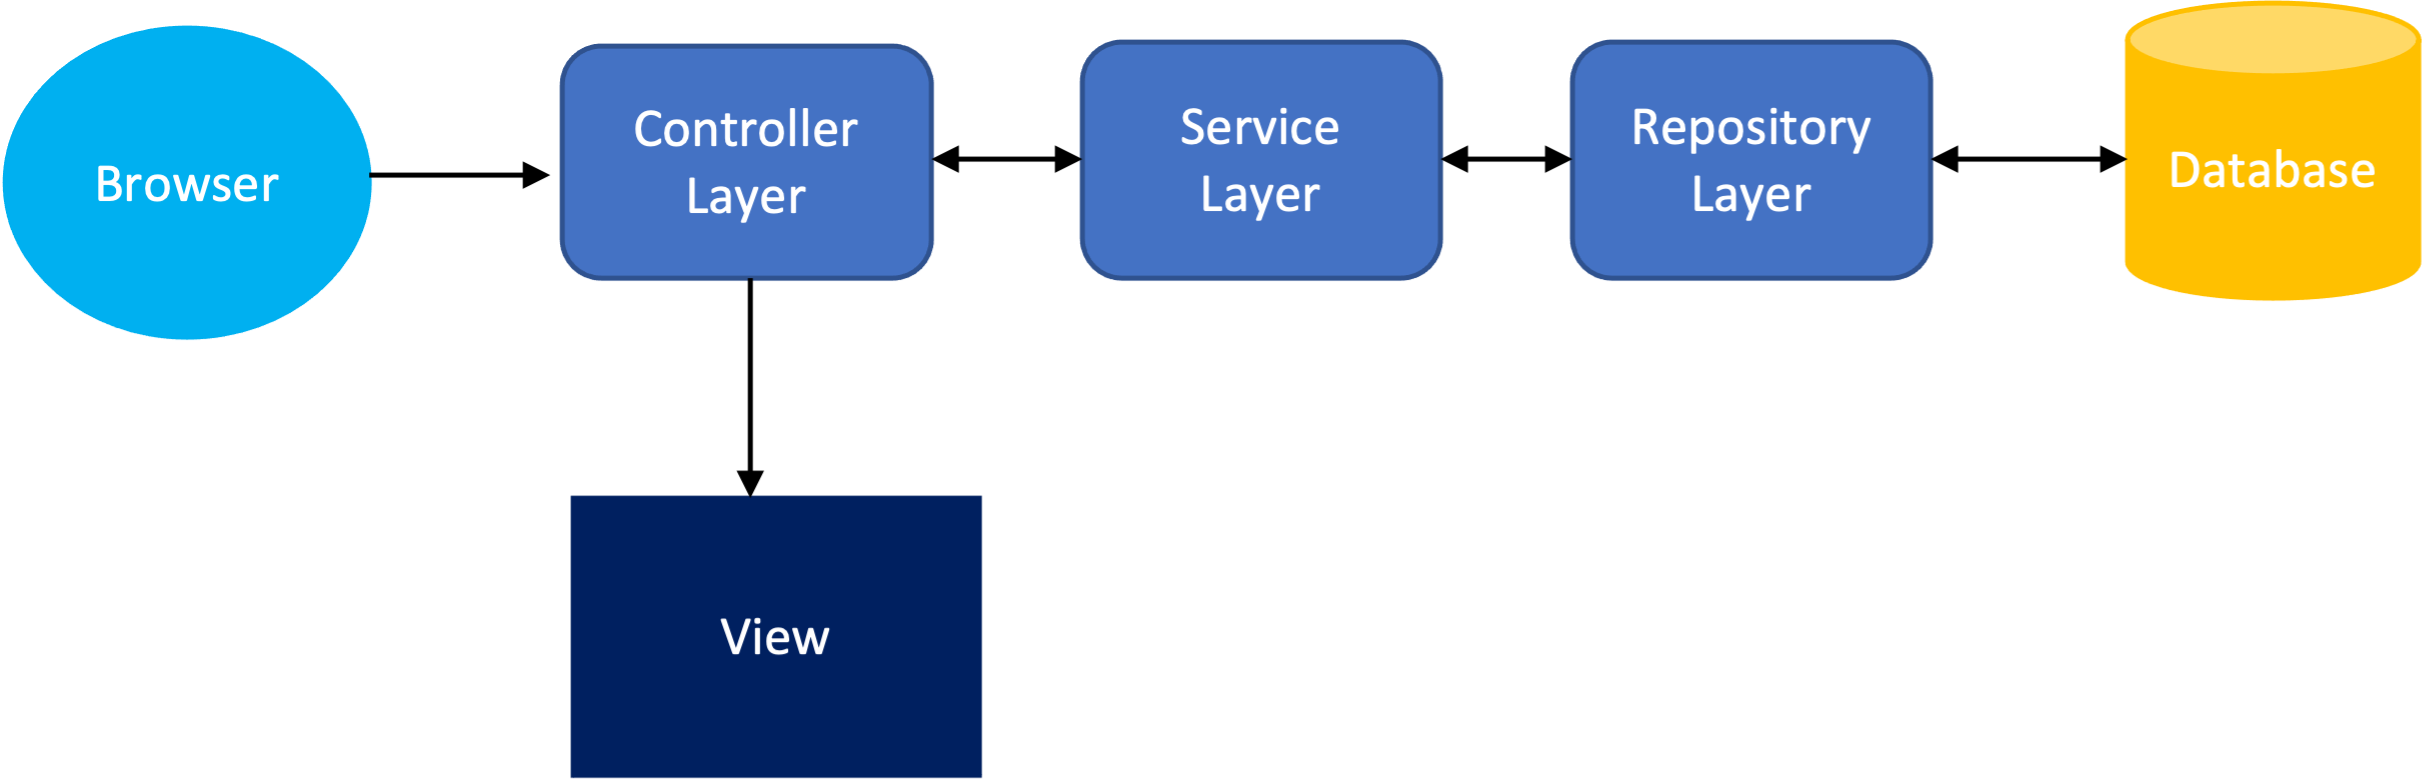
\includegraphics[width=\textwidth]{slike/mvc.png}
			\caption{MVC princip rada aplikacije}
			\label{fig:my_label}
		     \end{figure}
		
					\subsubsection{"front-end"}
					\textit{	U modelu klijent-poslužitelj, "klijentska strana aplikacije" odnosno dio web stranice s kojim korisnik(klijent) izravno komunicira naziva se front-end. Uključuje grafičko korisničko sučelje (GUI) odnosno sve što korisnici izravno doživljavaju: boje i stilove teksta, slike, grafikone i tablice, gumbe itd. Za izgradnju korisničkog sučelja odnosno front-enda koristimo alat React. }
					\bigskip 
					
					\subsubsection{"back-end"}
					\textit{	Poslužiteljska strana aplikacije pohranjuje i raspoređuje podatke te osigurava da sve na strani klijenta na web stranici radi dobro. To je dio web stranice koji korisnici ne mogu vidjeti i s njime ne mogu komunicirati odnosno to je ono što zovemo back-end. Za implementaciju back-enda koristimo Spring Boot zasnovan na razvojnom okviru Spring. }
				
	\newpage
	

		
		
		
		\section{Baza podataka}
		
		\textit{U bazi su kreirane relacije koje omogućavaju jednostavnu manipulaciju podacima (dodavanje, brisanje, izmjenjivanje i dohvat podataka). Sve relacije i entiteti uređeni su na 3. normalnu formu kako ne bi došlo do redundantnosti podataka. Da bi se lakše prikazala struktura korištene baze podataka, kreiran je relacijski dijagram baze podataka koji slijedi u nastavku. }
		
			\subsection{Dijagram baze podataka}	
		\begin{figure}[H]
			\centering
			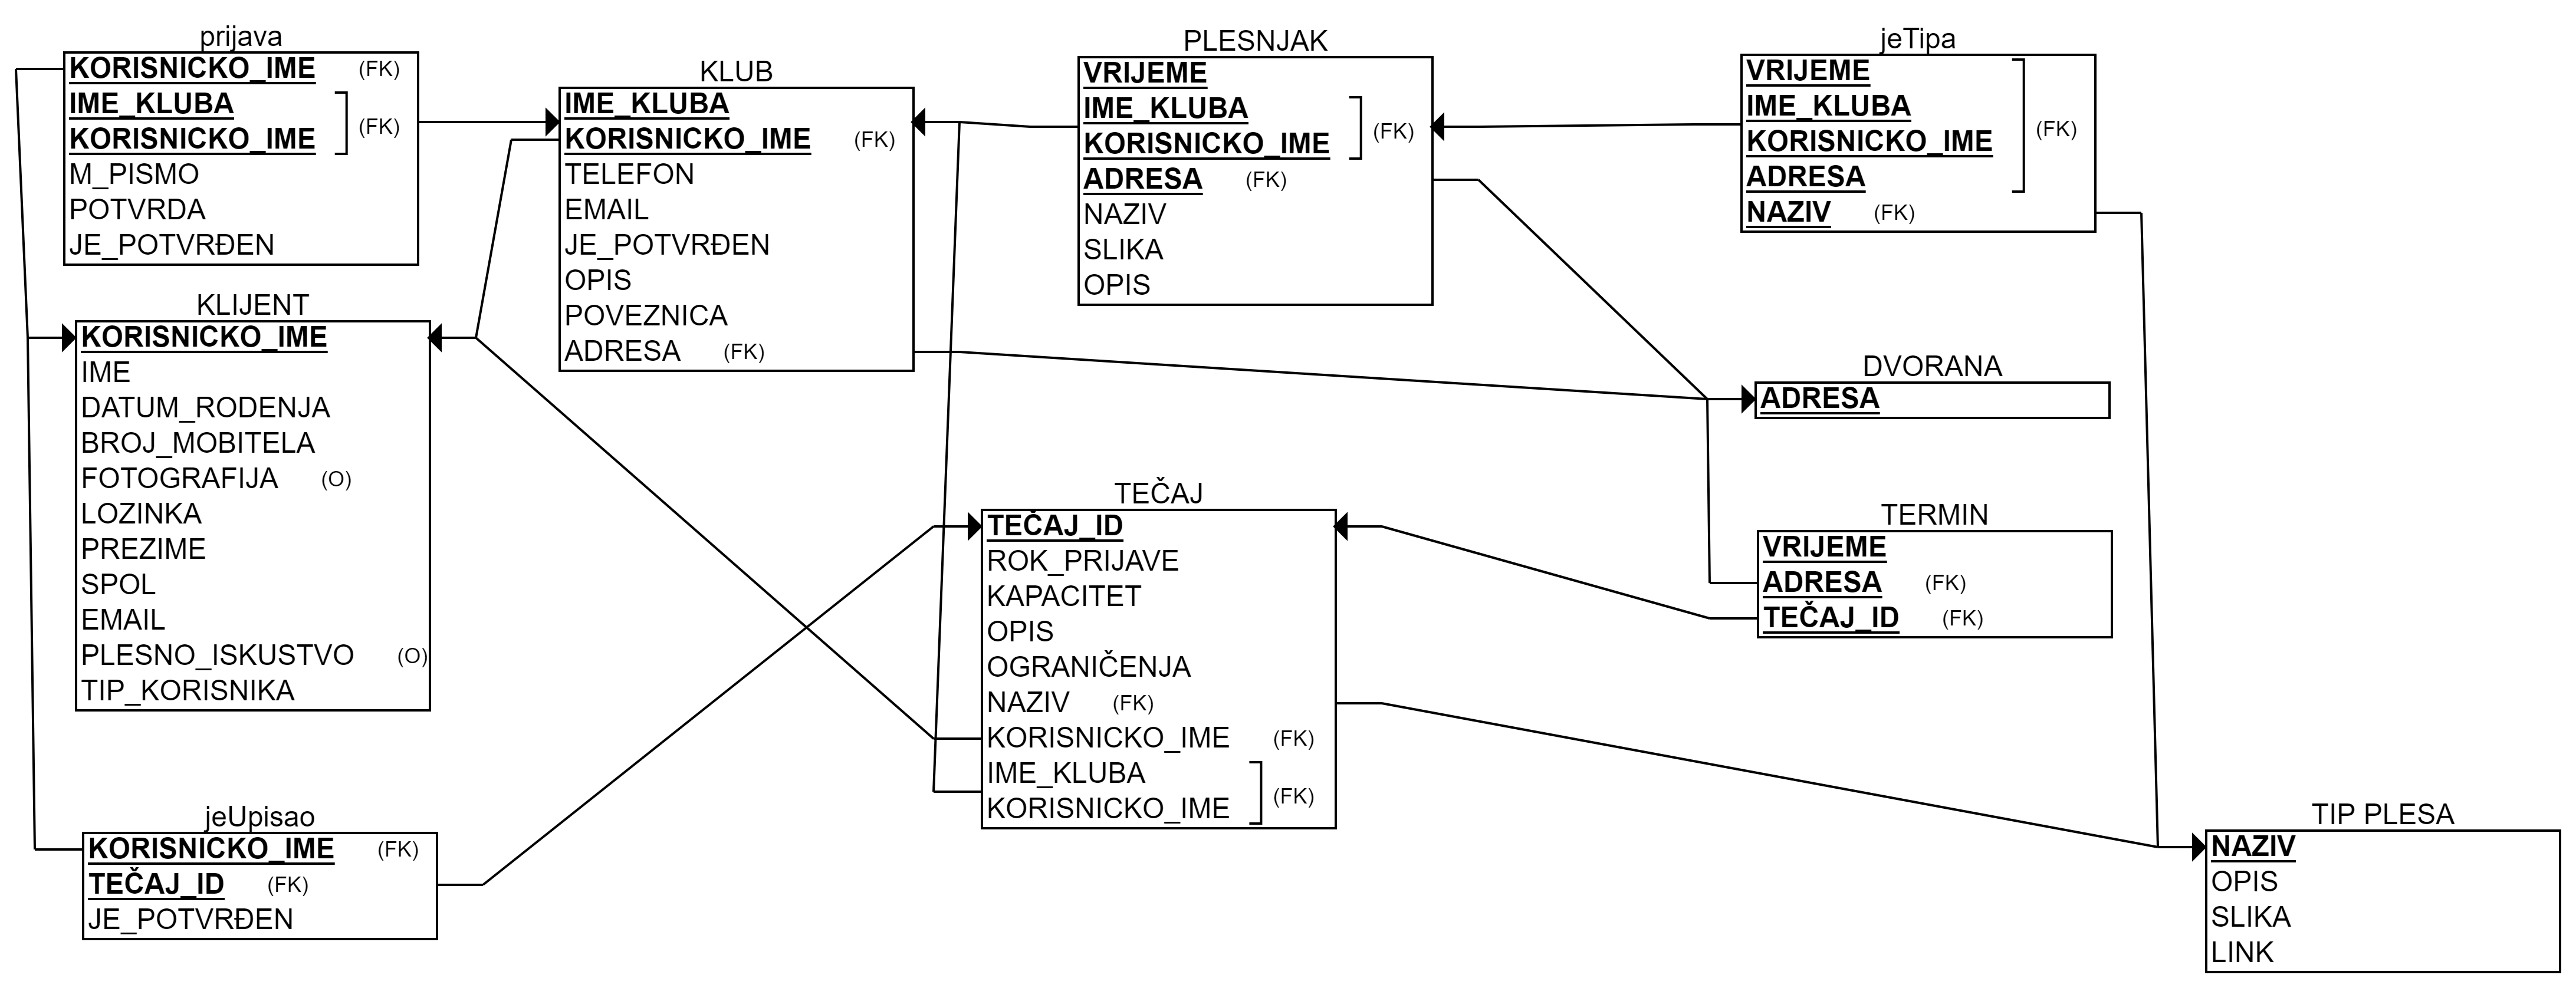
\includegraphics[width=\textwidth]{slike/baza.png}
			\caption{Relacijski dijagram baze podataka}
			\label{fig:my_label}
		\end{figure}
	
		
		\subsubsection{ Detaljnije o bazi }
		 Baza se sastoji od tablica (relacija) koje su definirane svojim imenom i skupom atributa. Baza podataka ove aplikacije sastoji se od sljedećih entiteta:
		 	\begin{packed_item}
		 		\item{Prijava}
		 		\item{Klijent}
		 		\item{JeUpisao}
		 		\item{Klub}
		 		\item{Plesnjak}
		 		\item{Tečaj}
		 		\item{jeTipa}
		 		\item{Dvorana}
		 		\item{Termin}
		 		\item{TipPlesa}
		 		
		 		\end{packed_item}
		 
		
		
			\subsection{Opis tablica}
			

				\textit{ Prva ćelija svake tablice označava njeno ime. U prvom stupcu navedeni su atributi tog entiteta, u drugom stupcu naveden je tip varijable, a u trećem opis svakog pojedinog atributa. Svjetlozelenom bojom označeni su primarni ključevi. Svjetlo plavom označeni su strani ključevi. Ukoliko je strani ključ također dio ključa, to je navedeno u opisu.}
				
				\subsubsection{Klijent}
				\textit{ Ovaj entitet  sadržava sve informacije o korisniku aplikacije kao što su korisničko ime, lozinka, ime, prezime, datum rođenja, broj mobitela, fotografija, spol, email, plesno iskustvo te koji je tip korisnika.}
				
				
				\begin{longtblr}[
					label=none,
					entry=none
					]{
						width = \textwidth,
						colspec={|X[12,l]|X[8, l]|X[20, l]|}, 
						rowhead = 1,
					} %definicija širine tablice, širine stupaca, poravnanje i broja redaka naslova tablice
					\hline \multicolumn{3}{|c|}{\textbf{KLIJENT}} & {\textbf{TIP}}	& {\textbf{OPIS}} \\ \hline[3pt]
					\SetCell{LightGreen}KORISNICKO\textunderscore IME & VARCHAR	&  Korisničko ime s kojim se korisnik prijavljuje	\\ \hline
					LOZINKA & VARCHAR	&  	Lozinka s kojom se korisnik prijavljuje	\\ \hline 
					IME	& VARCHAR &   Korisnikovo ime	\\ \hline 
					PREZIME & VARCHAR	&  Korisnikovo prezime		\\ \hline 
					DATUM\textunderscore RODENJA & DATE &  Korisnikov datum rođenja \\ \hline 
					BROJ\textunderscore MOBITELA & VARCHAR	&  	Korisnikov broj mobitela	\\ \hline 
					FOTOGRAFIJA & VARCHAR	&  	Put do korisnikove fotografije na serveru, OPCIONALNO	\\ \hline
					SPOL & VARCHAR(1)	&  	Korisnikov spol	\\ \hline
					EMAIL & VARCHAR	&  	Korisnikov email	\\ \hline  
					PLESNO\textunderscore ISKUSTVO & VARCHAR	&  	Opis korisikovog plesnog iskustva, OPCIONALNO	\\ \hline 
					TIP\textunderscore KORISNIKA & VARCHAR	&  	Jedan od: ADMINISTRATOR / VLASNIK KLUBA	\\ \hline 
				\end{longtblr}
			\newpage
			
			
			 \subsubsection{Dvorana}
			 \textit{Ovaj entitet sadržava informacije o plesnoj dvorani odnosno njenu adresu}
				
				\begin{longtblr}[
					label=none,
					entry=none
					]{
						width = \textwidth,
						colspec={|X[12,l]|X[8, l]|X[20, l]|}, 
						rowhead = 1,
					} %definicija širine tablice, širine stupaca, poravnanje i broja redaka naslova tablice
					\hline \multicolumn{3}{|c|}{\textbf{DVORANA}} & {\textbf{TIP}}	& {\textbf{OPIS}} \\ \hline[3pt]
					\SetCell{LightGreen}ADRESA & VARCHAR	&  Adresa plesne dvorane	\\ \hline
					
				\end{longtblr}
			\bigskip
			\bigskip
			
			  \subsubsection{Klub}
			 \textit{Ovaj entitet sadržava sve informacije koje su bitne za klub kao što su njegovo ime, korisnicko ime klijenta koji je vlasnik kluba, email od kluba, broj telefona od kluba, potvrdu o stanju (je li administrator potvrdio klub), opis kluba, poveznica na stranicu s grupama za upis te adresu kluba. }
			 	
	
				
				\begin{longtblr}[
					label=none,
					entry=none
					]{
						width = \textwidth,
						colspec={|X[12,l]|X[8, l]|X[20, l]|}, 
						rowhead = 1,
					} %definicija širine tablice, širine stupaca, poravnanje i broja redaka naslova tablice
					\hline \multicolumn{3}{|c|}{\textbf{KLUB}} & {\textbf{TIP}}	& {\textbf{OPIS}} \\ \hline[3pt]
					\SetCell{LightGreen}IME\textunderscore KLUBA & VARCHAR	&  Naziv kluba	\\ \hline
					\SetCell{LightBlue}KORISNICKO\textunderscore IME & VARCHAR	&  Dio ključa, korisničko ime klijenta koji je vlasnik kluba	\\ \hline
					EMAIL & VARCHAR	&  	Email od kluba	\\ \hline  
					TELEFON & VARCHAR	&  	Broj telefona od kluba	\\ \hline 
					JE\textunderscore POTVRĐEN & BOOLEAN	&  	Stanje je li administrator potvrdio klub	\\ \hline 
					OPIS	& VARCHAR &   Kratki opis kluba	\\ \hline 
					POVEZNICA & VARCHAR	&  	Poveznica na stranicu s grupama za upis	\\ \hline 
					\SetCell{LightBlue}ADRESA & VARCHAR	&  Adresa sjedišta kluba	\\ \hline
	
				\end{longtblr}
			\newpage
			
			 \subsubsection{Prijava}
			\textit{Ovaj entitet sadržava sve važne informacije korisnika koji ispunjava prijavu da postane  trener u klubu. Te informacije su navedene kao atributi : korisnicko ime trenera, ime kluba, korisnicko ime vlasnika kluba, motivacijsko pismo, potvrda korisnikove sposobnosti te stanje potvrde (je li vlasnik kluba potvrdio korisnika kao trenera). }
				
				\begin{longtblr}[
					label=none,
					entry=none
					]{
						width = \textwidth,
						colspec={|X[12,l]|X[8, l]|X[20, l]|}, 
						rowhead = 1,
					} %definicija širine tablice, širine stupaca, poravnanje i broja redaka naslova tablice
					\hline \multicolumn{3}{|c|}{\textbf{PRIJAVA}} & {\textbf{TIP}}	& {\textbf{OPIS}} \\ \hline[3pt]
					\SetCell{LightBlue}KORISNICKO\textunderscore IME TRENERA & VARCHAR	&  Dio ključa, korisničko ime klijenta koji želi postati trener	\\ \hline
					\SetCell{LightBlue}IME\textunderscore KLUBA & VARCHAR	&  Dio ključa, naziv kluba u kojem korisnik želi biti trener	\\ \hline
					\SetCell{LightBlue}KORISNICKO\textunderscore IME VLASNIKA & VARCHAR	&  Dio ključa, korisničko ime vlasnika kluba u kojem korisnik želi biti trener	\\ \hline
					
					M\textunderscore PISMO & VARCHAR	&  	Motivacijsko pismo trenera	\\ \hline  
					POTVRDA & VARCHAR	&  	Put do korisnikove potvrde sposobnosti, na serveru	\\ \hline  	
					JE\textunderscore POTVRDEN & BOOLEAN	&  	Stanje je li vlasnik kluba potvrdio trenera	\\ \hline  		
				\end{longtblr}
			\bigskip
			
			\subsubsection{Tip plesa}
			\textit{Ovaj entitet sadrži sve važne informacije o plesu, a to su : naziv, opis,slika, link }
			
				
					\begin{longtblr}[
					label=none,
					entry=none
					]{
						width = \textwidth,
						colspec={|X[12,l]|X[8, l]|X[20, l]|}, 
						rowhead = 1,
					} %definicija širine tablice, širine stupaca, poravnanje i broja redaka naslova tablice
					\hline \multicolumn{3}{|c|}{\textbf{TIP\textunderscore PLESA}} & {\textbf{TIP}}	& {\textbf{OPIS}} \\ \hline[3pt]
					\SetCell{LightGreen}NAZIV & VARCHAR	&  Ime plesa	\\ \hline
					
					OPIS & VARCHAR	&  	Kratki opis plesa	\\ \hline 
					SLIKA	& VARCHAR &   Put do slike plesa, na serveru	\\ \hline 
					LINK & VARCHAR	&  Link na videozapis plesa		\\ \hline 
					
				\end{longtblr}
			
			\newpage
			
				\subsubsection{Plesnjak}
			\textit{ Ovaj entitet sadrži sve važne informacije o održavanju plesnjaka kao što su vrijeme održavanja, ime kluba koji ga održava, korisničko ime vlasnika kluba koji organizira plesnjak, adresa održavanja plesnjaka, naziv plensjaka, slika i opis.}
			
			\begin{longtblr}[
				label=none,
				entry=none
				]{
					width = \textwidth,
					colspec={|X[12,l]|X[8, l]|X[20, l]|}, 
					rowhead = 1,
				} %definicija širine tablice, širine stupaca, poravnanje i broja redaka naslova tablice
				\hline \multicolumn{3}{|c|}{\textbf{PLESNJAK}} & {\textbf{TIP}}	& {\textbf{OPIS}} \\ \hline[3pt]
				\SetCell{LightGreen}VRIJEME & DATE	&  	Vrijeme održavanja plesnjaka\\ \hline
				\SetCell{LightBlue}IME\textunderscore KLUBA & VARCHAR	&  Dio ključa, naziv kluba koji organizira plesnjak	\\ \hline
				\SetCell{LightBlue}KORISNICKO\textunderscore IME & VARCHAR	&  Dio ključa, vlasnik kluba koji organizira plesnjak	\\ \hline
				\SetCell{LightBlue}ADRESA & VARCHAR	&  Dio ključa, mjesto održavanja plesnjaka	\\ \hline
				
				NAZIV & VARCHAR	&  	Naziv plesnjaka	\\ \hline  
				SLIKA & VARCHAR	&  	Put do slike o plesnjaku, na serveru	\\ \hline  
				OPIS	& VARCHAR &   Kratki opis plesnjaka	\\ \hline 
				
			\end{longtblr}
		
			\subsubsection{Termin}
		\textit{Ovaj entitet sadrži sve važne informacije o terminu održavanja određenog tečaja, a to je : vrijeme održavanja, adresa održavanja i ID tečaja koji se održava.}
		
		\begin{longtblr}[
			label=none,
			entry=none
			]{
				width = \textwidth,
				colspec={|X[12,l]|X[8, l]|X[20, l]|}, 
				rowhead = 1,
			} %definicija širine tablice, širine stupaca, poravnanje i broja redaka naslova tablice
			\hline \multicolumn{3}{|c|}{\textbf{TERMIN}} & {\textbf{TIP}}	& {\textbf{OPIS}} \\ \hline[3pt]
			\SetCell{LightGreen}VRIJEME & DATE	&  Vrijeme održavanja tečaja	\\ \hline
			\SetCell{LightBlue}ADRESA & VARCHAR	&  Dio ključa, adresa dvorane gdje se održava tečaj	\\ \hline
			\SetCell{LightBlue}TECAJ\textunderscore ID & INT	&  Dio ključa, ID tečaja koji se održava	\\ \hline
			
		\end{longtblr}
	
	\newpage
	
		
			\subsubsection{Plesnjak tipa}
		\textit{Ovaj entitet sadržava sve važne informacije o tipu plesnjaka koji postoji. Kako se na plesnjaku može plesati više vrsta plesova, ovdje su bitne informacije : vrijeme održavanja plesnjaka, ime kluba koji ga organizira, korisnicko ime vlasnika kluba, adresa održavanja i naziv plesa koji se pleše na plesnjaku.}
				
				\begin{longtblr}[
					label=none,
					entry=none
					]{
						width = \textwidth,
						colspec={|X[12,l]|X[8, l]|X[20, l]|}, 
						rowhead = 1,
					} %definicija širine tablice, širine stupaca, poravnanje i broja redaka naslova tablice
					\hline \multicolumn{3}{|c|}{\textbf{PLESNJAK\textunderscore TIPA}} & {\textbf{TIP}}	& {\textbf{OPIS}} \\ \hline[3pt]
					\SetCell{LightBlue}VRIJEME & DATE	&  Dio ključa, vrijeme održavanja plesnjaka	\\ \hline
					\SetCell{LightBlue}IME\textunderscore KLUBA & VARCHAR	&  Dio ključa, naziv kluba koji organizira plesnjak	\\ \hline
					\SetCell{LightBlue}KORISNICKO\textunderscore IME & VARCHAR	&  Dio ključa, vlasnik kluba koji organizira plesnjak	\\ \hline
					\SetCell{LightBlue}ADRESA & VARCHAR	&  Dio ključa, mjesto održavanja plesnjaka	\\ \hline
					\SetCell{LightBlue}NAZIV\textunderscore PLESA & VARCHAR	&  Dio ključa, naziv plesa koji se pleše na plesnjaku	\\ \hline
			
				\end{longtblr}
			\bigskip
			\bigskip
			
				\subsubsection{Upis tecaj}
			\textit{Ovaj entitet sadrži sve važne informacije o upisu klijenta na određeni tečaj, a to su : korisničko ime tog klijenta, ID tečaja koji se upisuje i stanje (je li upis potvrđen).}
			
			\begin{longtblr}[
				label=none,
				entry=none
				]{
					width = \textwidth,
					colspec={|X[12,l]|X[8, l]|X[20, l]|}, 
					rowhead = 1,
				} %definicija širine tablice, širine stupaca, poravnanje i broja redaka naslova tablice
				\hline \multicolumn{3}{|c|}{\textbf{UPIS\textunderscore TECAJ}} & {\textbf{TIP}}	& {\textbf{OPIS}} \\ \hline[3pt]
				\SetCell{LightBlue}KORISNICKO\textunderscore IME & VARCHAR	&  Dio ključa, korisničko ime klijenta	\\ \hline
				\SetCell{LightBlue}TECAJ\textunderscore ID & INT	&  Dio ključa, ID tečaja koji se upisuje	\\ \hline
				
				JE\textunderscore POTVRDEN & BOOLEAN	&  	Stanje je li korisnikov upis na tečaj potvrđen	\\ \hline 
			\end{longtblr}
			
			\newpage
			
			
				\subsubsection{Tecaj}
			\textit{Ovaj entitet sadržava sve važne informacije o pojedinom tečaju, a to su njegov ID, rok za prijavu na tečaj, kapacitet grupe na tečaju, kratki opis tečaja, ograničenja, naziv plesa za koji se tečaj održava, korisnicko ime trenera, ime kluba koji održava tečaj  te korisničko ime vlasnika tog kluba.}
				
				\begin{longtblr}[
					label=none,
					entry=none
					]{
						width = \textwidth,
						colspec={|X[12,l]|X[8, l]|X[20, l]|}, 
						rowhead = 1,
					} %definicija širine tablice, širine stupaca, poravnanje i broja redaka naslova tablice
					\hline \multicolumn{3}{|c|}{\textbf{TECAJ}} & {\textbf{TIP}}	& {\textbf{OPIS}} \\ \hline[3pt]
					\SetCell{LightGreen}TECAJ\textunderscore ID & INT	&  ID tečaja	\\ \hline
					ROK\textunderscore PRIJAVE & DATE	&  	Rok za prijavu	\\ \hline 
					KAPACITET	& INT &   Kapacitet grupe	\\ \hline 
					OPIS & VARCHAR	&  Kratki opis tečaja		\\ \hline 
					OGRANICENJA & VARCHAR &  Dodatne informacije i pravila ponašanja \\ \hline 
					\SetCell{LightBlue}NAZIV\textunderscore PLESA & VARCHAR	&  Naziv plesa za koji se održava tečaj	\\ \hline
					\SetCell{LightBlue}KORISNICKO\textunderscore IME TRENERA & VARCHAR	&  Korisničko ime trenera koji vodi tečaj	\\ \hline
					\SetCell{LightBlue}IME\textunderscore KLUBA & VARCHAR	&  Ime kluba koji održava tečaj	\\ \hline
					\SetCell{LightBlue}KORISNICKO\textunderscore IME VLASNIKA & VARCHAR	&  Korisničko ime vlasnika kluba koji održava tečaj	\\ \hline
					
					
				\end{longtblr}
			\newpage
			
			
		
			
		\section{Dijagram razreda}
		
			\textit{ Dijagramom razreda (klasa) prikazujemo razrede u sustavu, njihove atribute (članske varijable) i operacije (metode) te veze između razreda koji međusobno komuniciraju ili se nasljeđuju. Slike 4.5, 4.6 i 4.7 prikazuju dijagrame razreda po MVC arhitekturi aplikacije za lakše snalaženje. }
			\bigskip
			
			\textit{Slika 4.5 prikazuje razrede koji pripadaju Modelu. Svaki navedeni razred preslikava se u odgovarajuću tablicu u bazi. }
			\bigskip
			
			\textit{Slika 4.6 prikazuje razrede, točnije sučelja koja pripadaju sloju Repository.}
			\bigskip
			
			\textit{Slika 4.7 prikazuje sučelja i razrede koji implementiraju ta sučelja. Cijeli dio pripada sloju Service. Service komunicira sa Repository i Controller slojem.}
			\bigskip
			
				\textit{Slika 4.8 prikazuje razrede Controller sloja.}
			\bigskip
			
			
			\begin{figure}[H]
				\centering
				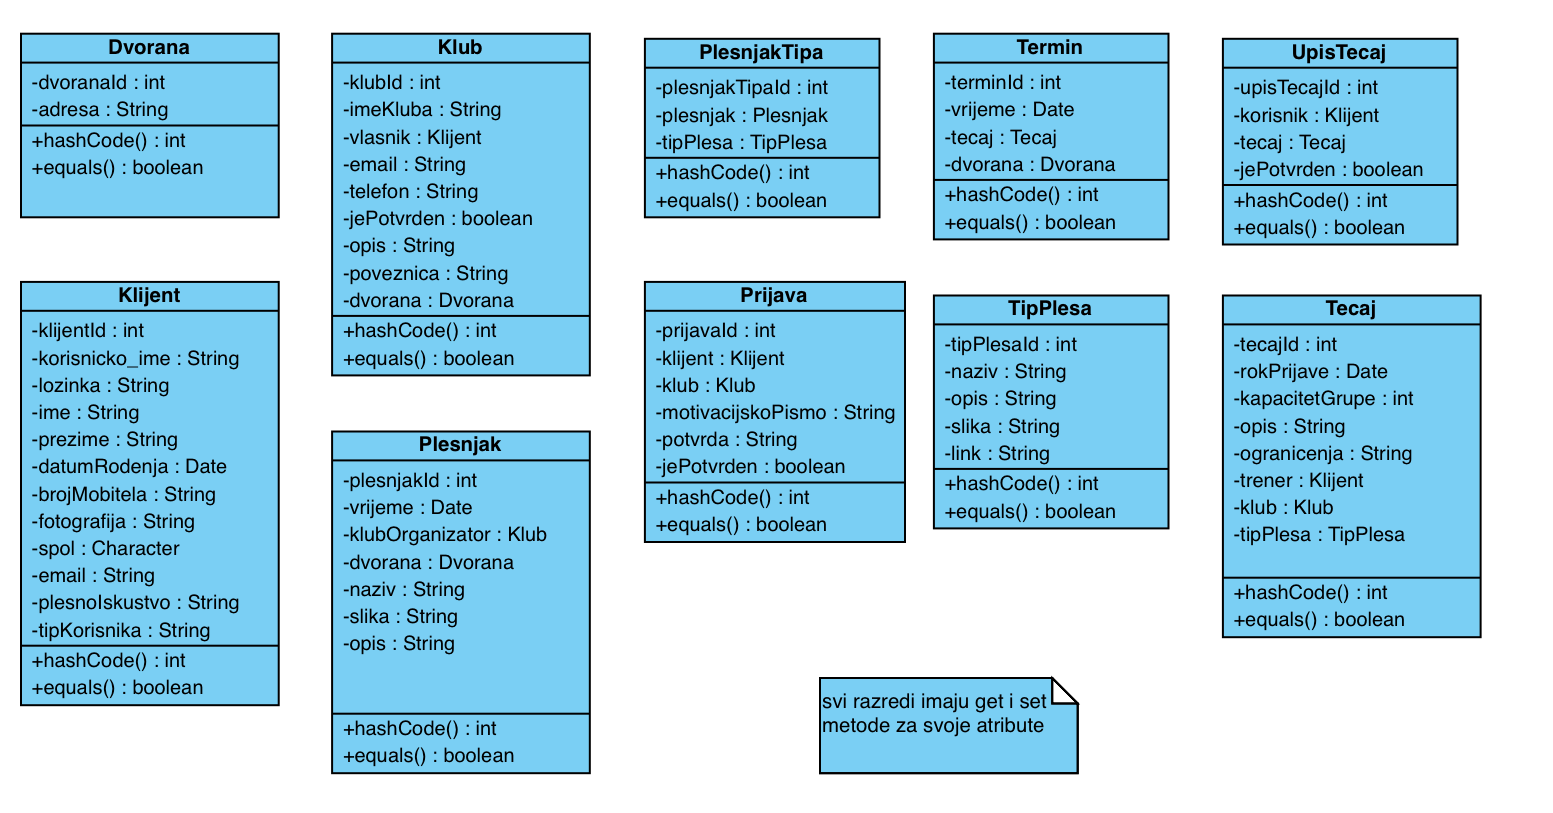
\includegraphics[width=\textwidth]{slike/dijagram_razreda/model.png}
				\caption{Dijagram razreda (Model)}
				\label{fig:my_label}
		    \end{figure}
	    	
	    	\begin{figure}[H]
	    		\centering
	    		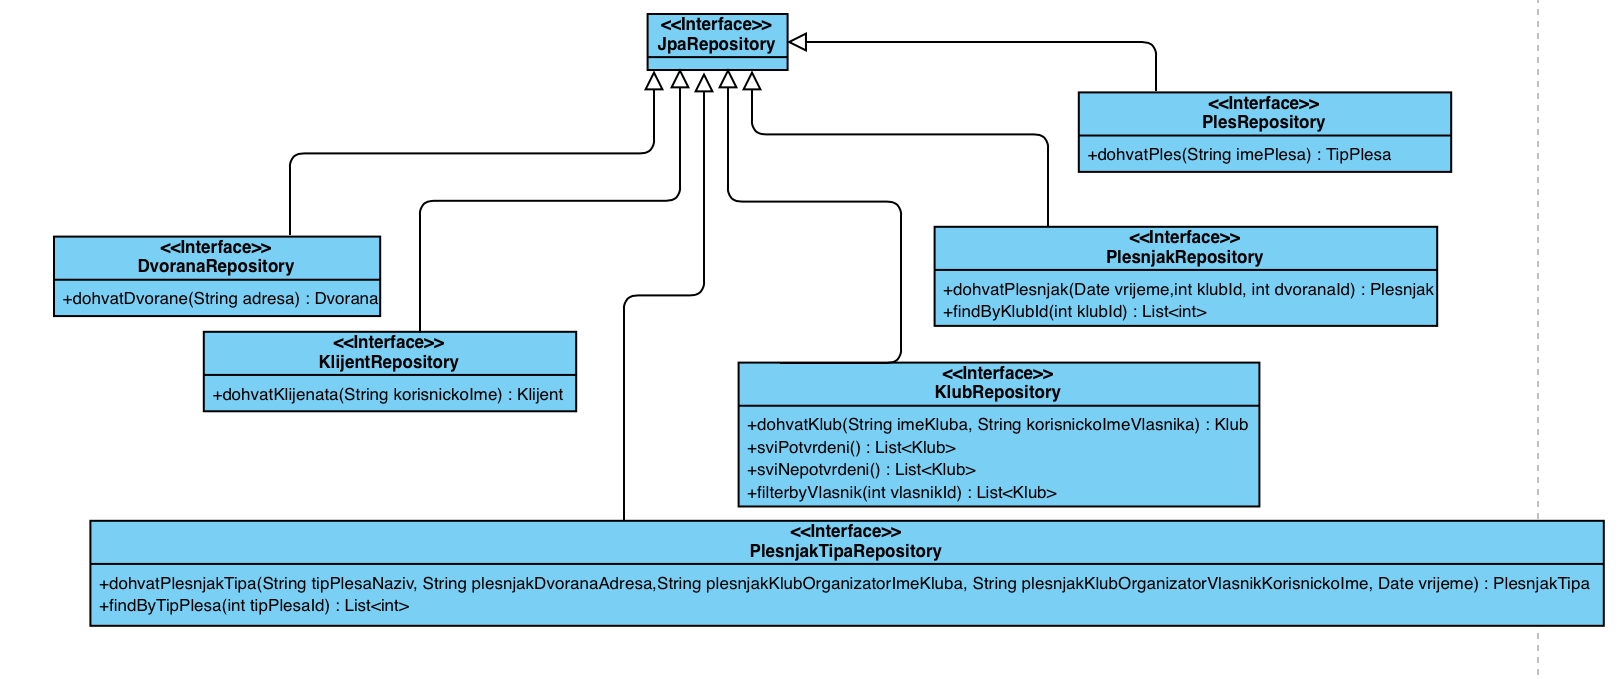
\includegraphics[width=\textwidth]{slike/dijagram_razreda/repository.png}
	    		\caption{Dijagram razreda (Repository)}
	    		\label{fig:my_label}
	    	\end{figure}
    	
    	\begin{figure}[H]
    		\centering
    		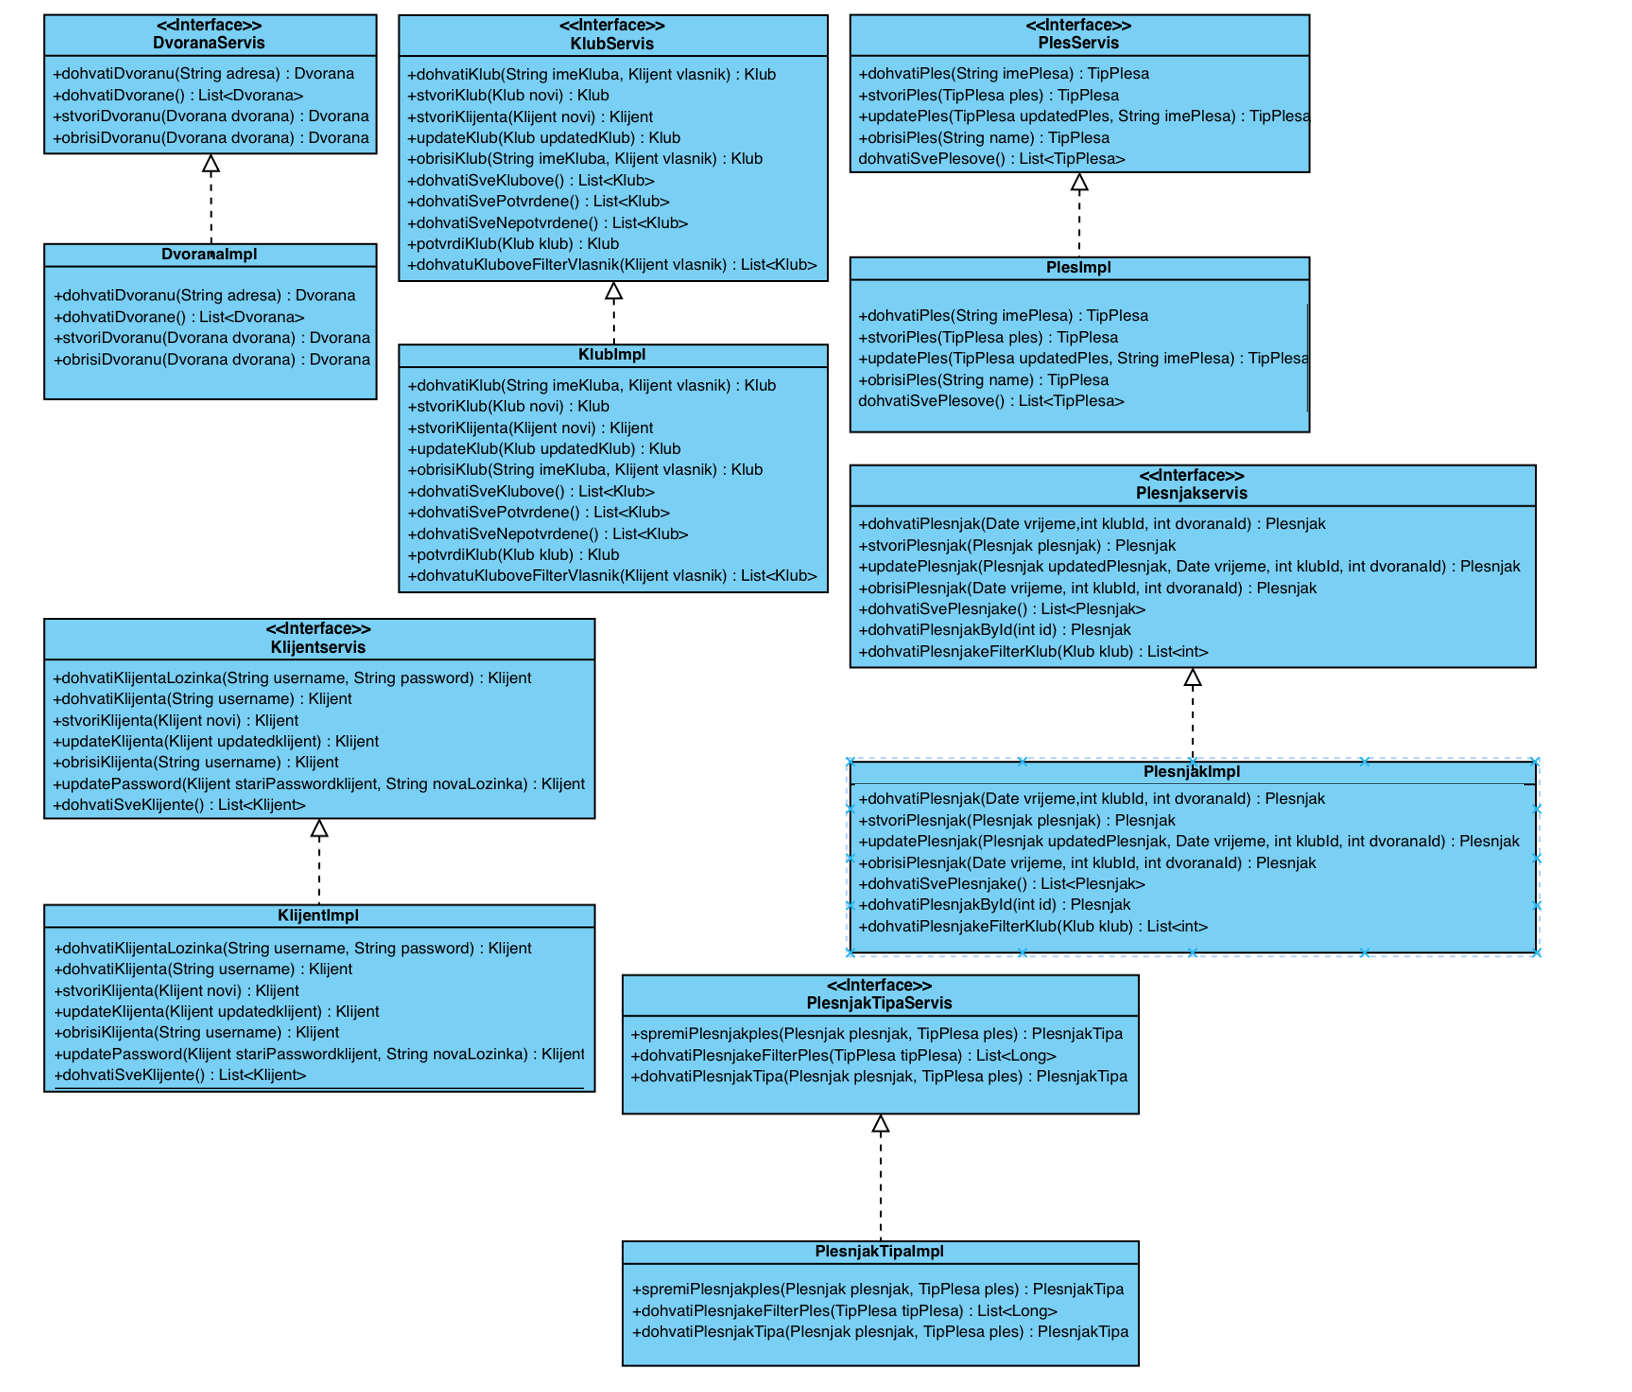
\includegraphics[width=\textwidth]{slike/dijagram_razreda/service.png}
    		\caption{Dijagram razreda (Service)}
    		\label{fig:my_label}
    	\end{figure}
    	
    	\begin{figure}[H]
    		\centering
    		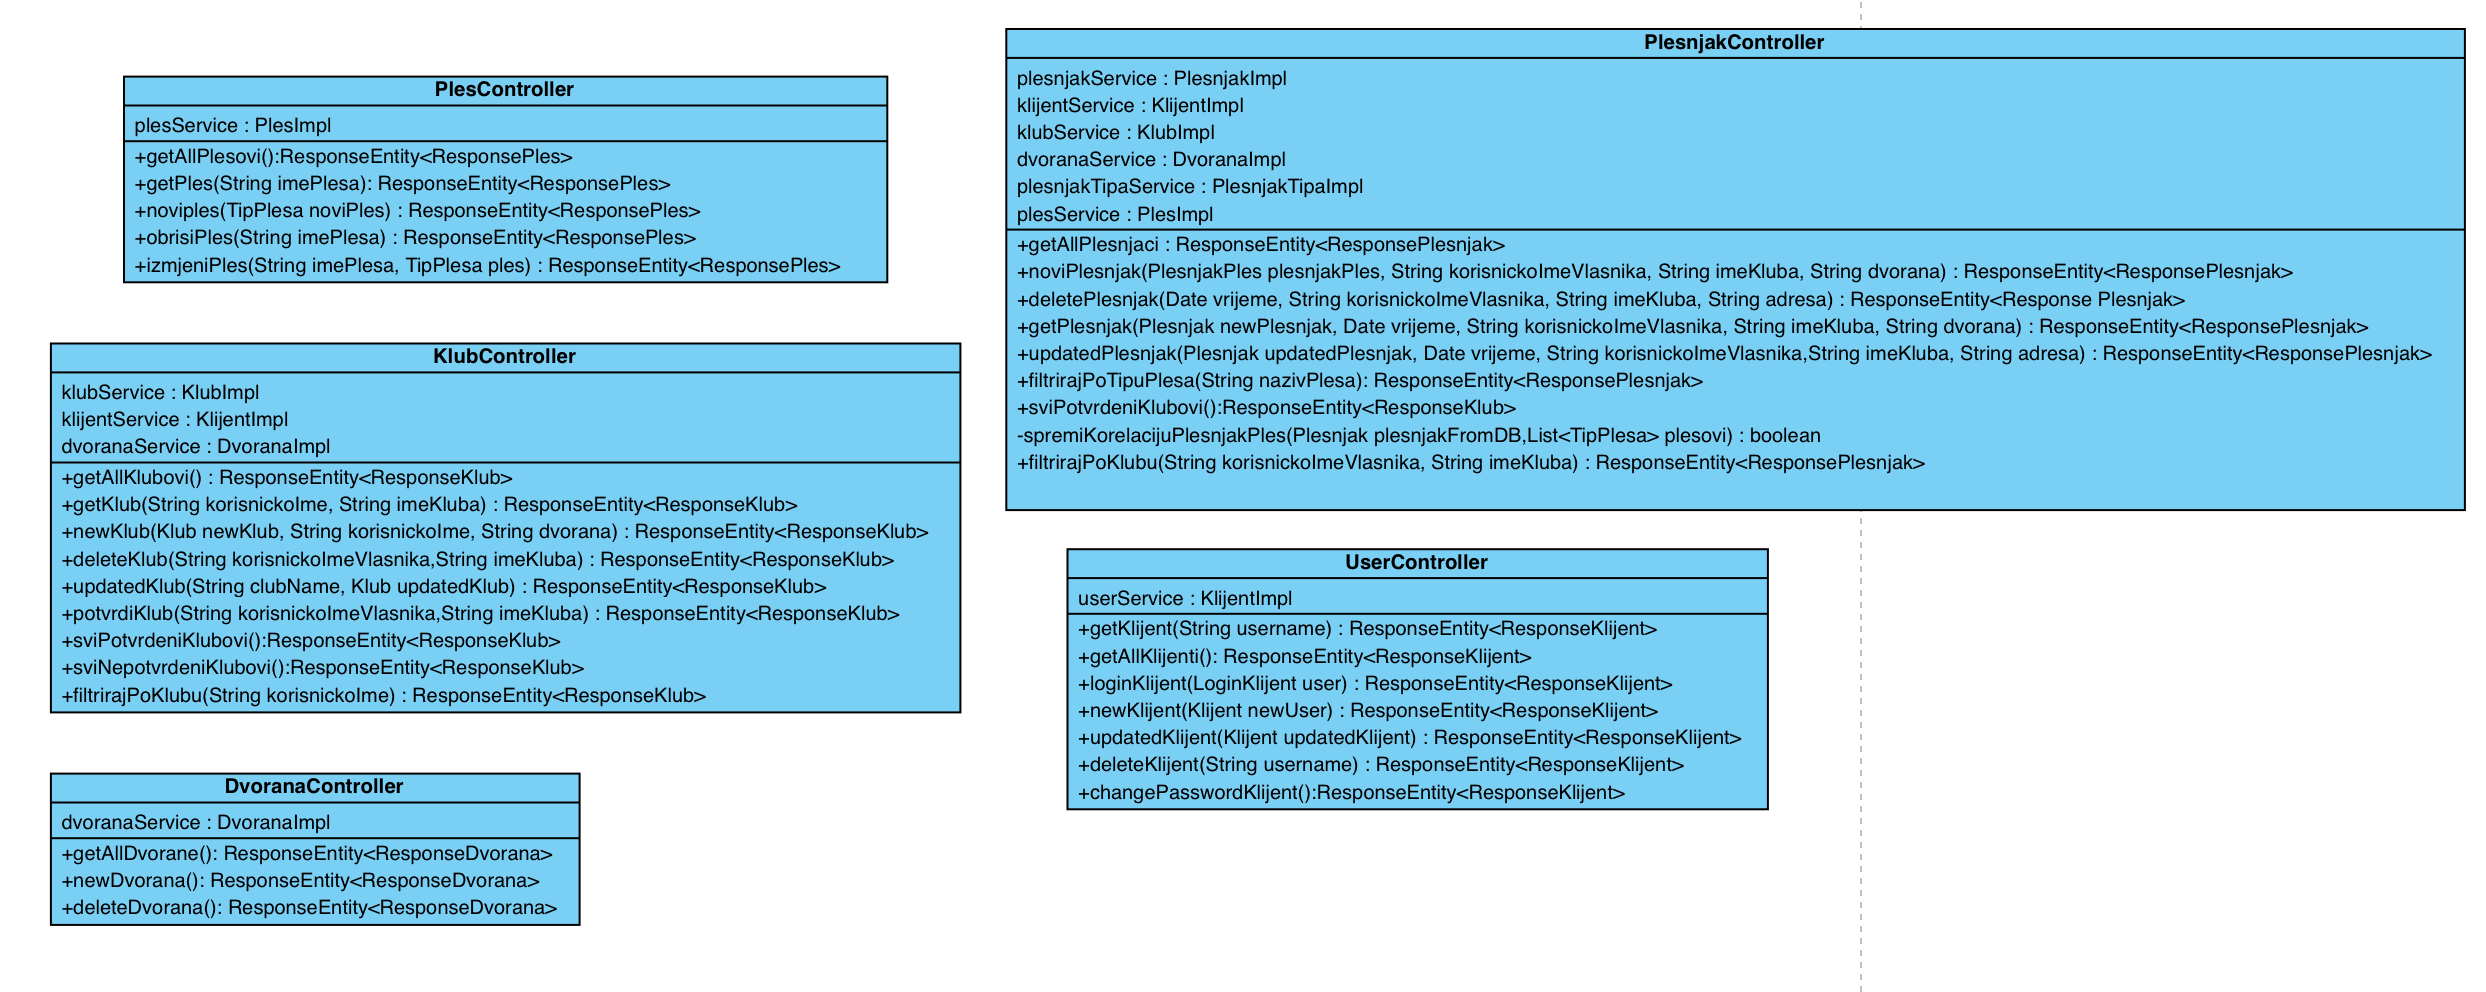
\includegraphics[width=\textwidth]{slike/dijagram_razreda/controller.png}
    		\caption{Dijagram razreda (Controller)}
    		\label{fig:my_label}
    	\end{figure}
			
	
			
			\section{Dijagram stanja}
			
			\textit{ Dijagram stanja prikazuje stanja objekta te prijelaze iz jednog stanja u drugo temeljene na događajima. Prilikom pokretanja aplikacije dolazi se na početnu stranicu (eng.Home page). Neregistrirani korisnik ima mogućnost registracije/prijave u sustav ili može ostati neregistriran. \linebreak \textbf{Slika 4.9} prikazuje dijagram stanja za registriranog korisnika. Nakon prijave, klijentu se prikazuje početna stranica na kojoj je karta s dostupnim plesnjacima i lokacijama klubova. Klikom na karticu „Profile“  klijentu je dostupan pregled profila. Klijent može pregledati, mijenjati osobne podatke i izbrisati korisnički račun. Odabirom kartice „My Clubs“ klijentu se pruža mogućnost registracije vlastitog kluba. Novo registrirani klubovi prvo moraju biti potvrđeni od strane administratora. Klikom na lokaciju kluba na karti otvara se profil kluba. Na stranici "profil kluba" korisnik može pregledati sve klubove, tečajeve, uređivati podatke ili izbrisati klub. Također može organizirati plesnjak ili postati trenerom za što postoje odgovarajuće forme. Ako je korisnik administrator onda može klikom na karticu "Admin" pregledati sve klijente, plesove i klubove. Može organizirati plesnjak, napraviti listu plesova te potvrđivati novonastale klubove.}
			
			\begin{figure}[H]
				\centering
				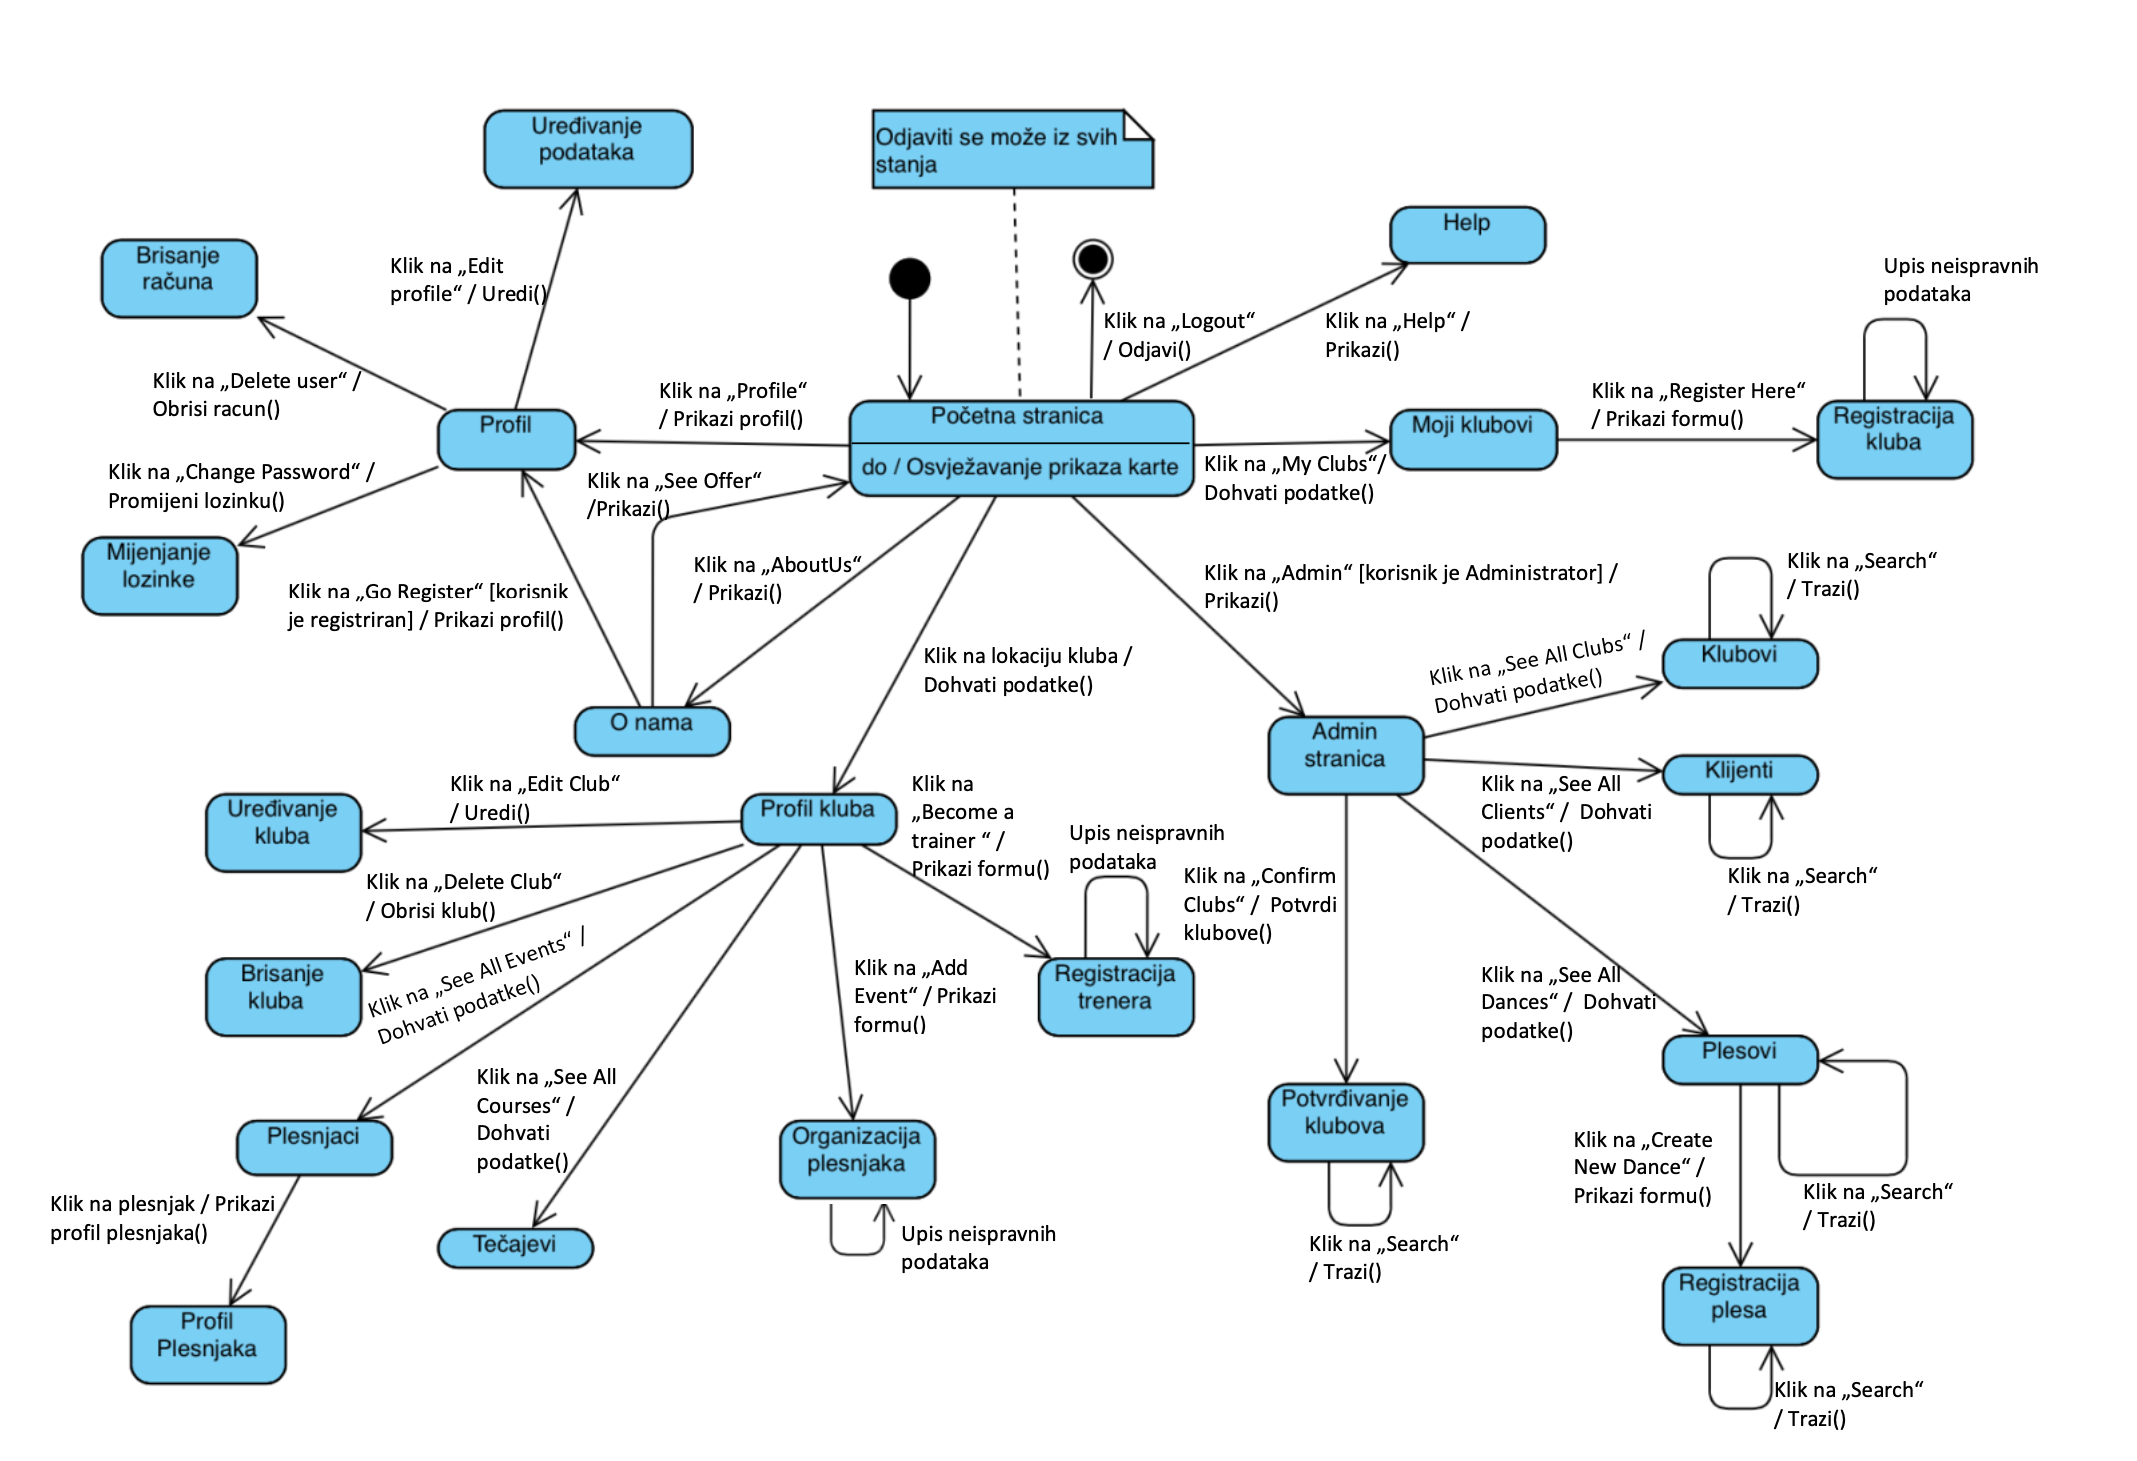
\includegraphics[width=\textwidth]{slike/dijagram_stanja.png}
				\caption{Dijagram stanja (Klijent)}
				\label{fig:my_label}
		   	\end{figure}
			
		
			
			\section{Dijagram aktivnosti}
	
			\textit{Dijagram aktivnosti opisuje model toka upravljanja ili toka podataka. Svaki novi korak obavlja se nakon završenog prethodnog. Slika 4.10 prikazuje dijagram aktivnosti za proces organizacije/stvaranja  plesnjaka. Korisnik se prijavi u sustav te mu se na početnoj stranici prikaže karta s klubovima. Odabire jedan klub za koji će stvoriti plesnjak. Otvara se stranica odabranog kluba na kojoj se pruža mogužnost stvaranja plesnjaka. Kada korisnik  upiše odgovarajuće podatke, na stranici profila kluba nalazi se lista novostvorenih plesnjaka. }
			
			\begin{figure}[H]
			\centering
			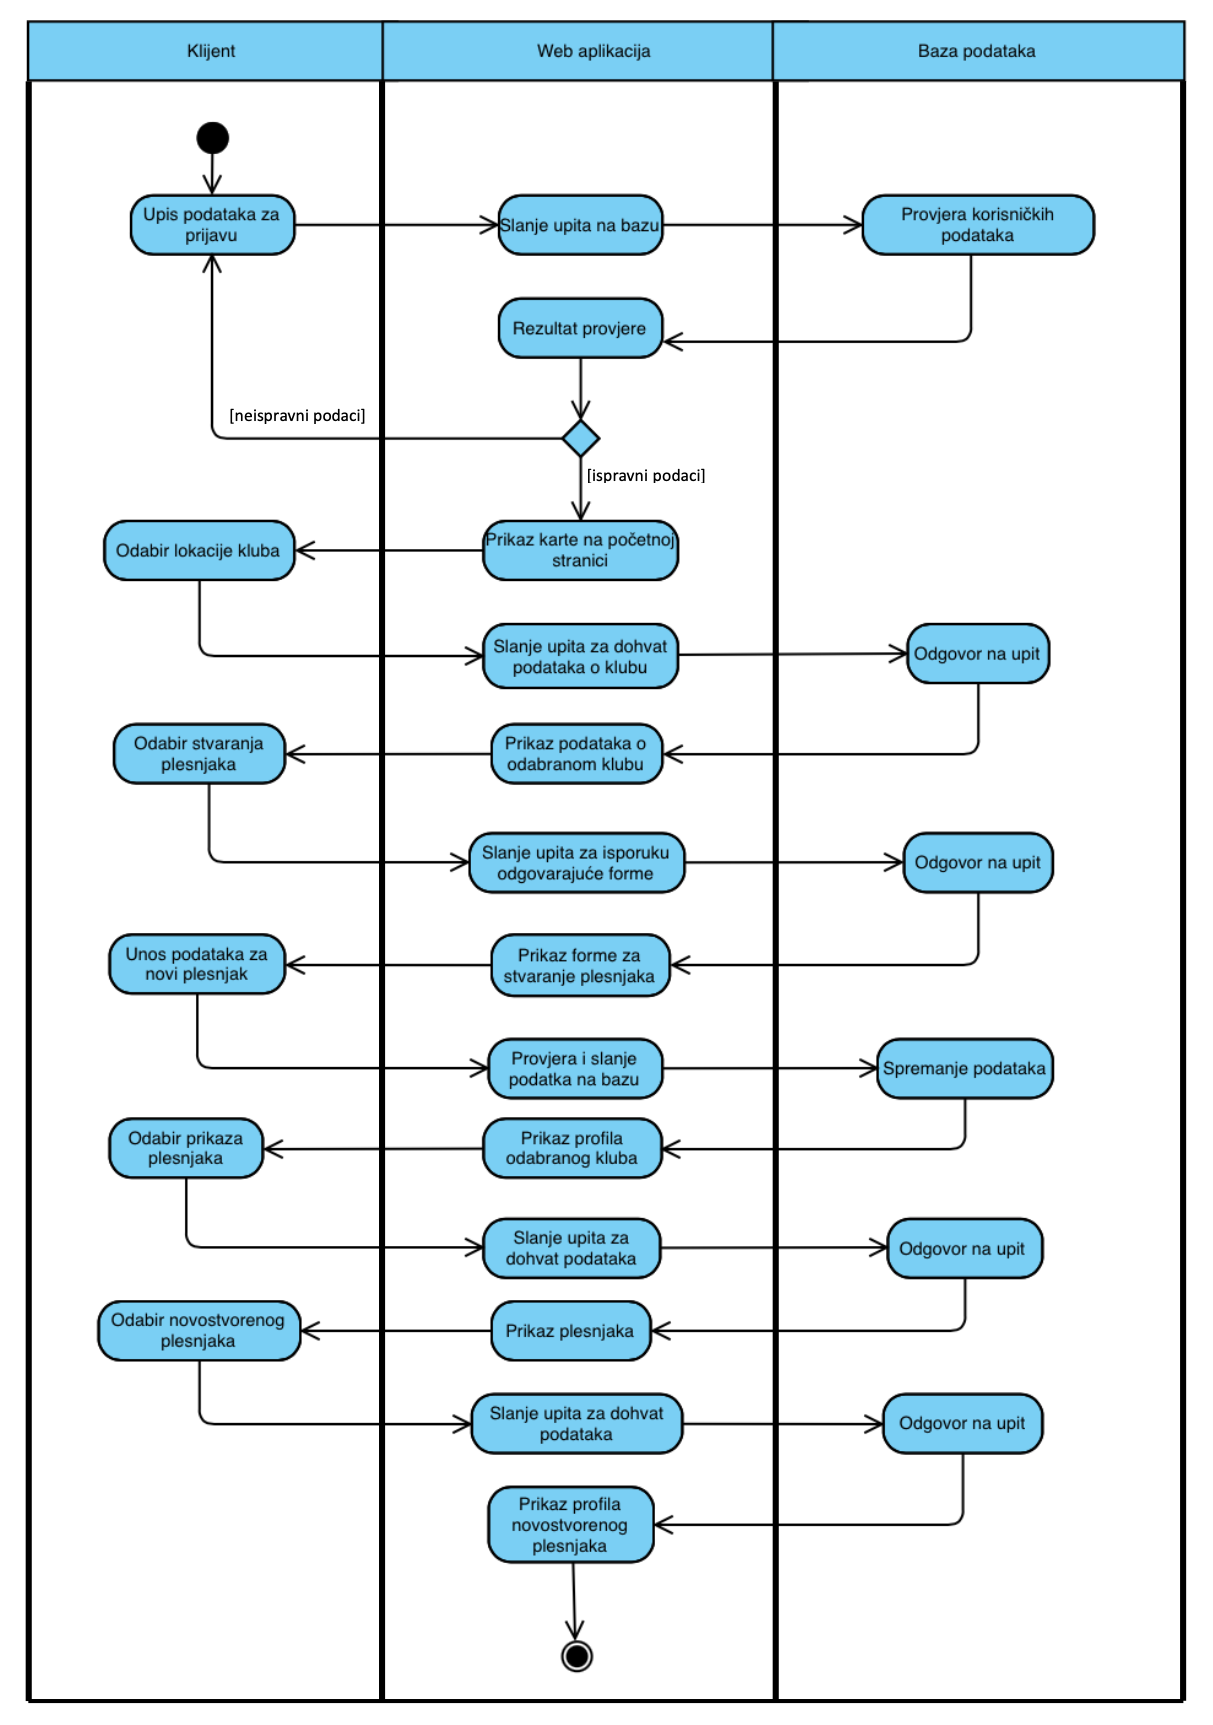
\includegraphics[width=\textwidth]{slike/dijagram_aktivnosti.png}
			\caption{Dijagram aktivnosti(Organizacija plesnjaka)}
			\label{fig:my_label}
	     	\end{figure}
	 	\eject 
			
			
			\section{Dijagram komponenti}
			\textit{Dijagram komponenti opisuje organizaciju i međuovisnost komponenti, interne strukture i odnose prema okolini. Prikazan je kao frontend i backend aplikacija koje su integrirane REST API-jem.}
			
			\textit{Backend aplikacija sastoji se od modela, servisa, repozitorija i kontrolera. Model nam služi za organizaciju podataka koji će se spremati u bazu. Repozitorij komunicira s bazom podataka (SQL upiti) za dohvaćanje podataka koji su nam potrebni. Servis komunicira sa repozitorijem i kontrolerom. Kontroler obrađuje dolazne zahtjev (zahtjeve sa frontenda). }
			\textit{Frontend aplikacija se sastoji od routera, komponenti, servisa te raznih biblioteka. Router je komponenta koja na korisnikov upit za određeni url određuje koja će se datoteka (stranica) isporučiti. Komponente su stranice koje se isporučuju odnosno to su javascript datoteke (html, css, javascript kod) koje ovise o React biblioteci.  Servisi nam ovdje služe za pozive prema backendu, validacije i slično. Axios je biblioteka HTTP klijenta koja olakšava slanje HTTP zahtjeva na REST API (odnosno slanje zahtjeva na backend aplikaciju). }
		
		
			\begin{figure}[H]
				\centering
				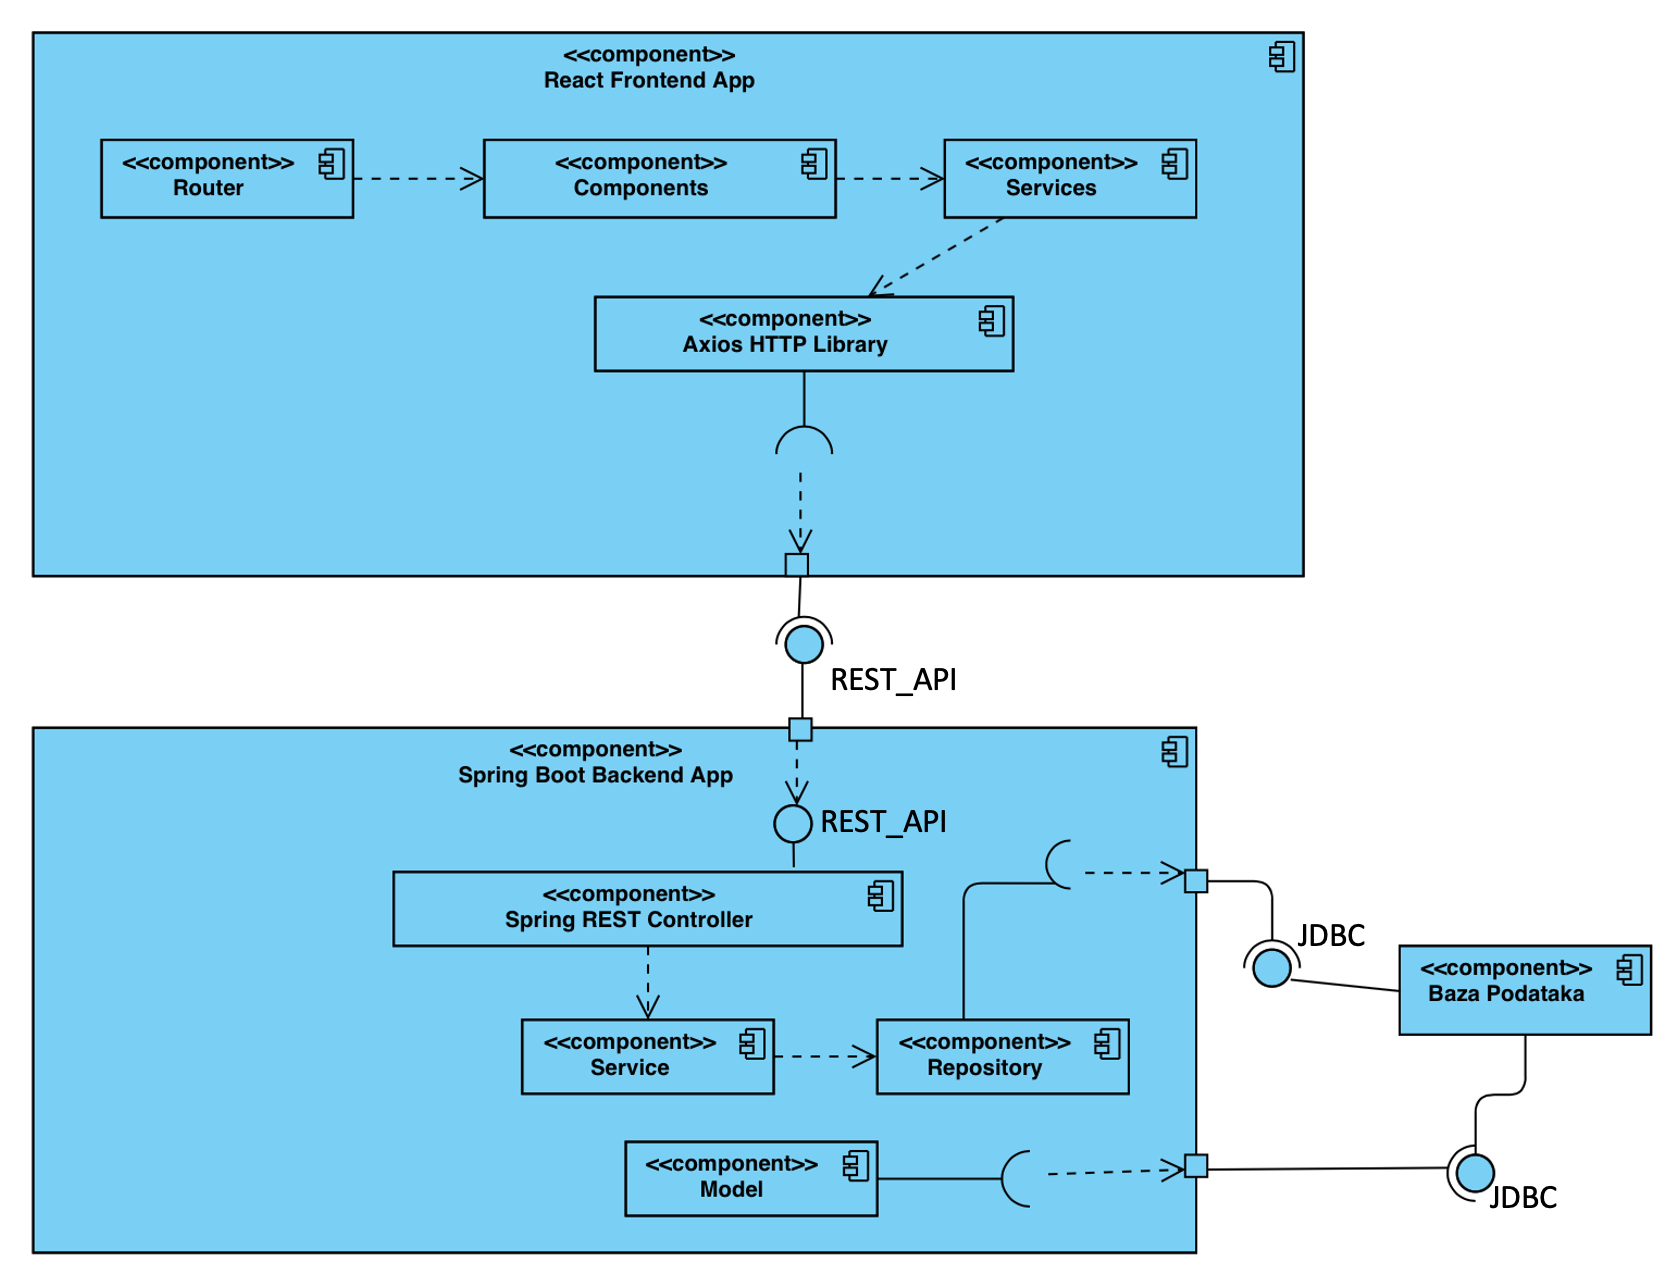
\includegraphics[width=\textwidth]{slike/dijagram_komponenti.png}
				\caption{Dijagram komponenti}
				\label{fig:my_label}
			\end{figure}
			
			
			
			
			